\documentclass[]{article}
\usepackage[left=1in,top=1in,right=1in,bottom=1in]{geometry}


%%%% more monte %%%%
% thispagestyle{empty}
% https://stackoverflow.com/questions/2166557/how-to-hide-the-page-number-in-latex-on-first-page-of-a-chapter
\usepackage{color}
% \usepackage[table]{xcolor} % are they using color?

% \definecolor{WSU.crimson}{HTML}{981e32}
% \definecolor{WSU.gray}{HTML}{5e6a71}

% \definecolor{shadecolor}{RGB}{248,248,248}
\definecolor{WSU.crimson}{RGB}{152,30,50} % use http://colors.mshaffer.com to convert from 981e32
\definecolor{WSU.gray}{RGB}{94,106,113}

%%%%%%%%%%%%%%%%%%%%%%%%%%%%

\newcommand*{\authorfont}{\fontfamily{phv}\selectfont}
\usepackage{lmodern}


  \usepackage[T1]{fontenc}
  \usepackage[utf8]{inputenc}




\usepackage{abstract}
\renewcommand{\abstractname}{}    % clear the title
\renewcommand{\absnamepos}{empty} % originally center

\renewenvironment{abstract}
 {{%
    \setlength{\leftmargin}{0mm}
    \setlength{\rightmargin}{\leftmargin}%
  }%
  \relax}
 {\endlist}

\makeatletter
\def\@maketitle{%
  \pagestyle{empty}
  \newpage
%  \null
%  \vskip 2em%
%  \begin{center}%
  \let \footnote \thanks
    {\fontsize{18}{20}\selectfont\raggedright  \setlength{\parindent}{0pt} \@title \par}%
}
%\fi
\makeatother






\usepackage{color}
\usepackage{fancyvrb}
\newcommand{\VerbBar}{|}
\newcommand{\VERB}{\Verb[commandchars=\\\{\}]}
\DefineVerbatimEnvironment{Highlighting}{Verbatim}{commandchars=\\\{\}}
% Add ',fontsize=\small' for more characters per line
\usepackage{framed}
\definecolor{shadecolor}{RGB}{248,248,248}
\newenvironment{Shaded}{\begin{snugshade}}{\end{snugshade}}
\newcommand{\AlertTok}[1]{\textcolor[rgb]{0.94,0.16,0.16}{#1}}
\newcommand{\AnnotationTok}[1]{\textcolor[rgb]{0.56,0.35,0.01}{\textbf{\textit{#1}}}}
\newcommand{\AttributeTok}[1]{\textcolor[rgb]{0.77,0.63,0.00}{#1}}
\newcommand{\BaseNTok}[1]{\textcolor[rgb]{0.00,0.00,0.81}{#1}}
\newcommand{\BuiltInTok}[1]{#1}
\newcommand{\CharTok}[1]{\textcolor[rgb]{0.31,0.60,0.02}{#1}}
\newcommand{\CommentTok}[1]{\textcolor[rgb]{0.56,0.35,0.01}{\textit{#1}}}
\newcommand{\CommentVarTok}[1]{\textcolor[rgb]{0.56,0.35,0.01}{\textbf{\textit{#1}}}}
\newcommand{\ConstantTok}[1]{\textcolor[rgb]{0.00,0.00,0.00}{#1}}
\newcommand{\ControlFlowTok}[1]{\textcolor[rgb]{0.13,0.29,0.53}{\textbf{#1}}}
\newcommand{\DataTypeTok}[1]{\textcolor[rgb]{0.13,0.29,0.53}{#1}}
\newcommand{\DecValTok}[1]{\textcolor[rgb]{0.00,0.00,0.81}{#1}}
\newcommand{\DocumentationTok}[1]{\textcolor[rgb]{0.56,0.35,0.01}{\textbf{\textit{#1}}}}
\newcommand{\ErrorTok}[1]{\textcolor[rgb]{0.64,0.00,0.00}{\textbf{#1}}}
\newcommand{\ExtensionTok}[1]{#1}
\newcommand{\FloatTok}[1]{\textcolor[rgb]{0.00,0.00,0.81}{#1}}
\newcommand{\FunctionTok}[1]{\textcolor[rgb]{0.00,0.00,0.00}{#1}}
\newcommand{\ImportTok}[1]{#1}
\newcommand{\InformationTok}[1]{\textcolor[rgb]{0.56,0.35,0.01}{\textbf{\textit{#1}}}}
\newcommand{\KeywordTok}[1]{\textcolor[rgb]{0.13,0.29,0.53}{\textbf{#1}}}
\newcommand{\NormalTok}[1]{#1}
\newcommand{\OperatorTok}[1]{\textcolor[rgb]{0.81,0.36,0.00}{\textbf{#1}}}
\newcommand{\OtherTok}[1]{\textcolor[rgb]{0.56,0.35,0.01}{#1}}
\newcommand{\PreprocessorTok}[1]{\textcolor[rgb]{0.56,0.35,0.01}{\textit{#1}}}
\newcommand{\RegionMarkerTok}[1]{#1}
\newcommand{\SpecialCharTok}[1]{\textcolor[rgb]{0.00,0.00,0.00}{#1}}
\newcommand{\SpecialStringTok}[1]{\textcolor[rgb]{0.31,0.60,0.02}{#1}}
\newcommand{\StringTok}[1]{\textcolor[rgb]{0.31,0.60,0.02}{#1}}
\newcommand{\VariableTok}[1]{\textcolor[rgb]{0.00,0.00,0.00}{#1}}
\newcommand{\VerbatimStringTok}[1]{\textcolor[rgb]{0.31,0.60,0.02}{#1}}
\newcommand{\WarningTok}[1]{\textcolor[rgb]{0.56,0.35,0.01}{\textbf{\textit{#1}}}}



\title{\textbf{\textcolor{WSU.crimson}{The Modern Vitruvian
Man}} \newline \textbf{\textcolor{WSU.gray}{Body Proportions}}  }
 

%  

% \author{ \Large true \hfill \normalsize \emph{} }
\author{\Large Nathan
Shine\vspace{0.05in} \newline\normalsize\emph{Washington State
University}  }


\date{December 14, 2020}
\setcounter{secnumdepth}{3}

\usepackage{titlesec}
% See the link above: KOMA classes are not compatible with titlesec any more. Sorry.
% https://github.com/jbezos/titlesec/issues/11
\titleformat*{\section}{\bfseries}
\titleformat*{\subsection}{\bfseries\itshape}
\titleformat*{\subsubsection}{\itshape}
\titleformat*{\paragraph}{\itshape}
\titleformat*{\subparagraph}{\itshape}

% https://code.usgs.gov/usgs/norock/irvine_k/ip-092225/


%\titleformat*{\section}{\normalsize\bfseries}
%\titleformat*{\subsection}{\normalsize\itshape}
%\titleformat*{\subsubsection}{\normalsize\itshape}
%\titleformat*{\paragraph}{\normalsize\itshape}
%\titleformat*{\subparagraph}{\normalsize\itshape}

% https://tex.stackexchange.com/questions/233866/one-column-multicol-environment#233904
\usepackage{environ}
\NewEnviron{auxmulticols}[1]{%
  \ifnum#1<2\relax% Fewer than 2 columns
    %\vspace{-\baselineskip}% Possible vertical correction
    \BODY
  \else% More than 1 column
    \begin{multicols}{#1}
      \BODY
    \end{multicols}%
  \fi
}





\usepackage{natbib}
\setcitestyle{aysep={}} %% no year, comma just year
% \usepackage[numbers]{natbib}
\bibliographystyle{./../biblio/ormsv080.bst}



\usepackage[strings]{underscore} % protect underscores in most circumstances




\newtheorem{hypothesis}{Hypothesis}
\usepackage{setspace}


%%%%%%%%%%%%%%%%%%%%%%%%%%%%%%%%%%%%%%%%%%%%%%%%%%%%%
%%% MONTE ADDS %%%

\usepackage{fancyhdr} % fancy header 
\usepackage{lastpage} % last page 

\usepackage{multicol}


\usepackage{etoolbox}
\AtBeginEnvironment{quote}{\singlespacing\small}
% https://tex.stackexchange.com/questions/325695/how-to-style-blockquote


\usepackage{soul}			%% allows strike-through
\usepackage{url}			%% fixes underscores in urls
\usepackage{csquotes}		%% allows \textquote in references
\usepackage{rotating}		%% allows table and box rotation
\usepackage{caption}		%% customize caption information
\usepackage{booktabs}		%% enhance table/tabular environment
\usepackage{tabularx}		%% width attributes updates tabular
\usepackage{enumerate}		%% special item environment
\usepackage{enumitem}		%% special item environment

\usepackage{lineno}		%% allows linenumbers for editing using \linenumbers
\usepackage{hanging}


\usepackage{mathtools}  	%% also loads amsmath
\usepackage{bm}		%% bold-math
\usepackage{scalerel}	%% scale one element (make one beta bigger font)

\newcommand{\gFrac}[2]{ \genfrac{}{}{0pt}{1}{{#1}}{#2} }

\newcommand{\betaSH}[3]{  \gFrac{\text{\tiny #1}}{{\text{\tiny #2}}}\hat{\beta}_{\text{#3}}   }
\newcommand{\betaSB}[3]{              ^{\text{#1}} _{\text{#2}} \bm{\beta} _{\text{#3}}                   }  %% bold
\newcommand{\bigEQ}{  \scaleobj{1.5}{{\ }= } }
\newcommand{\bigP}[1]{  \scaleobj{1.5}{#1 } }





\usepackage{endnotes}  % he already does this ...
\renewcommand{\enotesize}{\normalsize}
% https://tex.stackexchange.com/questions/99984/endnotes-do-not-be-superscript-and-add-a-space
\renewcommand\makeenmark{\textsuperscript{[\theenmark]}} % in brackets %
% https://tex.stackexchange.com/questions/31574/how-to-control-the-indent-in-endnotes
\patchcmd{\enoteformat}{1.8em}{0pt}{}{}

\patchcmd{\theendnotes}
  {\makeatletter}
  {\makeatletter\renewcommand\makeenmark{\textbf{[\theenmark]} }}
  {}{}



% https://tex.stackexchange.com/questions/141906/configuring-footnote-position-and-spacing

\addtolength{\footnotesep}{5mm} % change to 1mm

\renewcommand{\thefootnote}{\textbf{\arabic{footnote}}}
\let\footnote=\endnote
%\renewcommand*{\theendnote}{\alph{endnote}}
%\renewcommand{\theendnote}{\textbf{\arabic{endnote}}}


\renewcommand*{\notesname}{ENDNOTES}

\makeatletter
\def\enoteheading{\section*{\notesname
  \@mkboth{\MakeUppercase{\notesname}}{\MakeUppercase{\notesname}}}%
  \mbox{}\par\vskip-2.3\baselineskip\noindent\rule{.5\textwidth}{0.4pt}\par\vskip\baselineskip}
\makeatother


\renewcommand*{\contentsname}{TABLE OF CONTENTS}

\renewcommand*{\refname}{REFERENCES}


%\usepackage{subfigure}
\usepackage{subcaption}

\captionsetup{labelfont=bf}  % Make Table / Figure bold

%%% you could add elements here ... monte says .... %%%
%\usepackage{mypackageForCapitalH}


%%%%%%%%%%%%%%%%%%%%%%%%%%%%%%%%%%%%%%%%%%%%%%%%%%%%%

% set default figure placement to htbp
\makeatletter
\def\fps@figure{htbp}
\makeatother


% move the hyperref stuff down here, after header-includes, to allow for - \usepackage{hyperref}

\makeatletter
\@ifpackageloaded{hyperref}{}{%
\ifxetex
  \PassOptionsToPackage{hyphens}{url}\usepackage[setpagesize=false, % page size defined by xetex
              unicode=false, % unicode breaks when used with xetex
              xetex]{hyperref}
\else
  \PassOptionsToPackage{hyphens}{url}\usepackage[draft,unicode=true]{hyperref}
\fi
}

\@ifpackageloaded{color}{
    \PassOptionsToPackage{usenames,dvipsnames}{color}
}{%
    \usepackage[usenames,dvipsnames]{color}
}
\makeatother
\hypersetup{breaklinks=true,
            bookmarks=true,
            pdfauthor={Nathan Shine (Washington State University)},
             pdfkeywords = {t-tests; proportions; data collection;
correlation investigation},  
            pdftitle={The Modern Vitruvian Man: Body Proportions},
            colorlinks=true,
            citecolor=blue,
            urlcolor=blue,
            linkcolor=magenta,
            pdfborder={0 0 0}}
\urlstyle{same}  % don't use monospace font for urls

% Add an option for endnotes. -----

%
% add tightlist ----------
\providecommand{\tightlist}{%
\setlength{\itemsep}{0pt}\setlength{\parskip}{0pt}}

% add some other packages ----------

% \usepackage{multicol}
% This should regulate where figures float
% See: https://tex.stackexchange.com/questions/2275/keeping-tables-figures-close-to-where-they-are-mentioned
\usepackage[section]{placeins}



\pagestyle{fancy}   
\lhead{\textcolor{WSU.crimson}{\textbf{ The Modern Vitruvian Man }}}
\chead{}
\rhead{\textcolor{WSU.gray}{\textbf{  Page\ \thepage\ of\ \protect\pageref{LastPage} }}}
\lfoot{}
\cfoot{}
\rfoot{}


\begin{document}
	
% \pagenumbering{arabic}% resets `page` counter to 1 
%    

% \maketitle

{% \usefont{T1}{pnc}{m}{n}
\setlength{\parindent}{0pt}
\thispagestyle{plain}
{\fontsize{18}{20}\selectfont\raggedright 
\maketitle  % title \par  

}

{
   \vskip 13.5pt\relax \normalsize\fontsize{11}{12} 
   
\textbf{\authorfont Nathan Shine} \hskip 15pt \emph{\small Washington
State University}   

}

}








\begin{abstract}

    \hbox{\vrule height .2pt width 39.14pc}

    \vskip 8.5pt % \small 

\noindent In this article we look at the measurements of the body as a
proportion of height. We compare the measurements gathered by students
to the ideal proportions set out by the Roman architect Vitruvius. We
also look at if females can fit within these proportions, and which
measurements can be used in place of height to explain
proportions\vspace{0.25in}

\noindent We find that the knee height, foot length, hand length, and
arm span proportions all line up with the Vitruvian proportions. Male
and female proportions do not differ greatly except for foot length. The
hand length proportion can also explain much of the other
proprtions.\vspace{0.25in}


\vskip 8.5pt \noindent \textbf{\underline{Keywords}:} t-tests;
proportions; data collection; correlation investigation \par

    




    
    \hbox{\vrule height .2pt width 39.14pc}
    \vskip 5pt 
    \hfill \textbf{\textcolor{WSU.gray}{ December 14, 2020 } }
    \vskip 5pt 
    
\end{abstract}


\vskip -8.5pt



 % removetitleabstract

\noindent  

\section{Introduction}
\label{sec:intro}

The Vitruvian Man was designed with certain proportions in mind.
Vitruvius was a Roman architect and in his writings he describes the
human body as a set of proportions of one's height. In this graphic we
can see which of our measurements aligned with the Vitruvian
proportions.

\begin{figure}[!ht]
    \centering
    %  trim={<left> <lower> <right> <upper>}
    % https://shantoroy.com/latex/add-subfig-in-latex/
            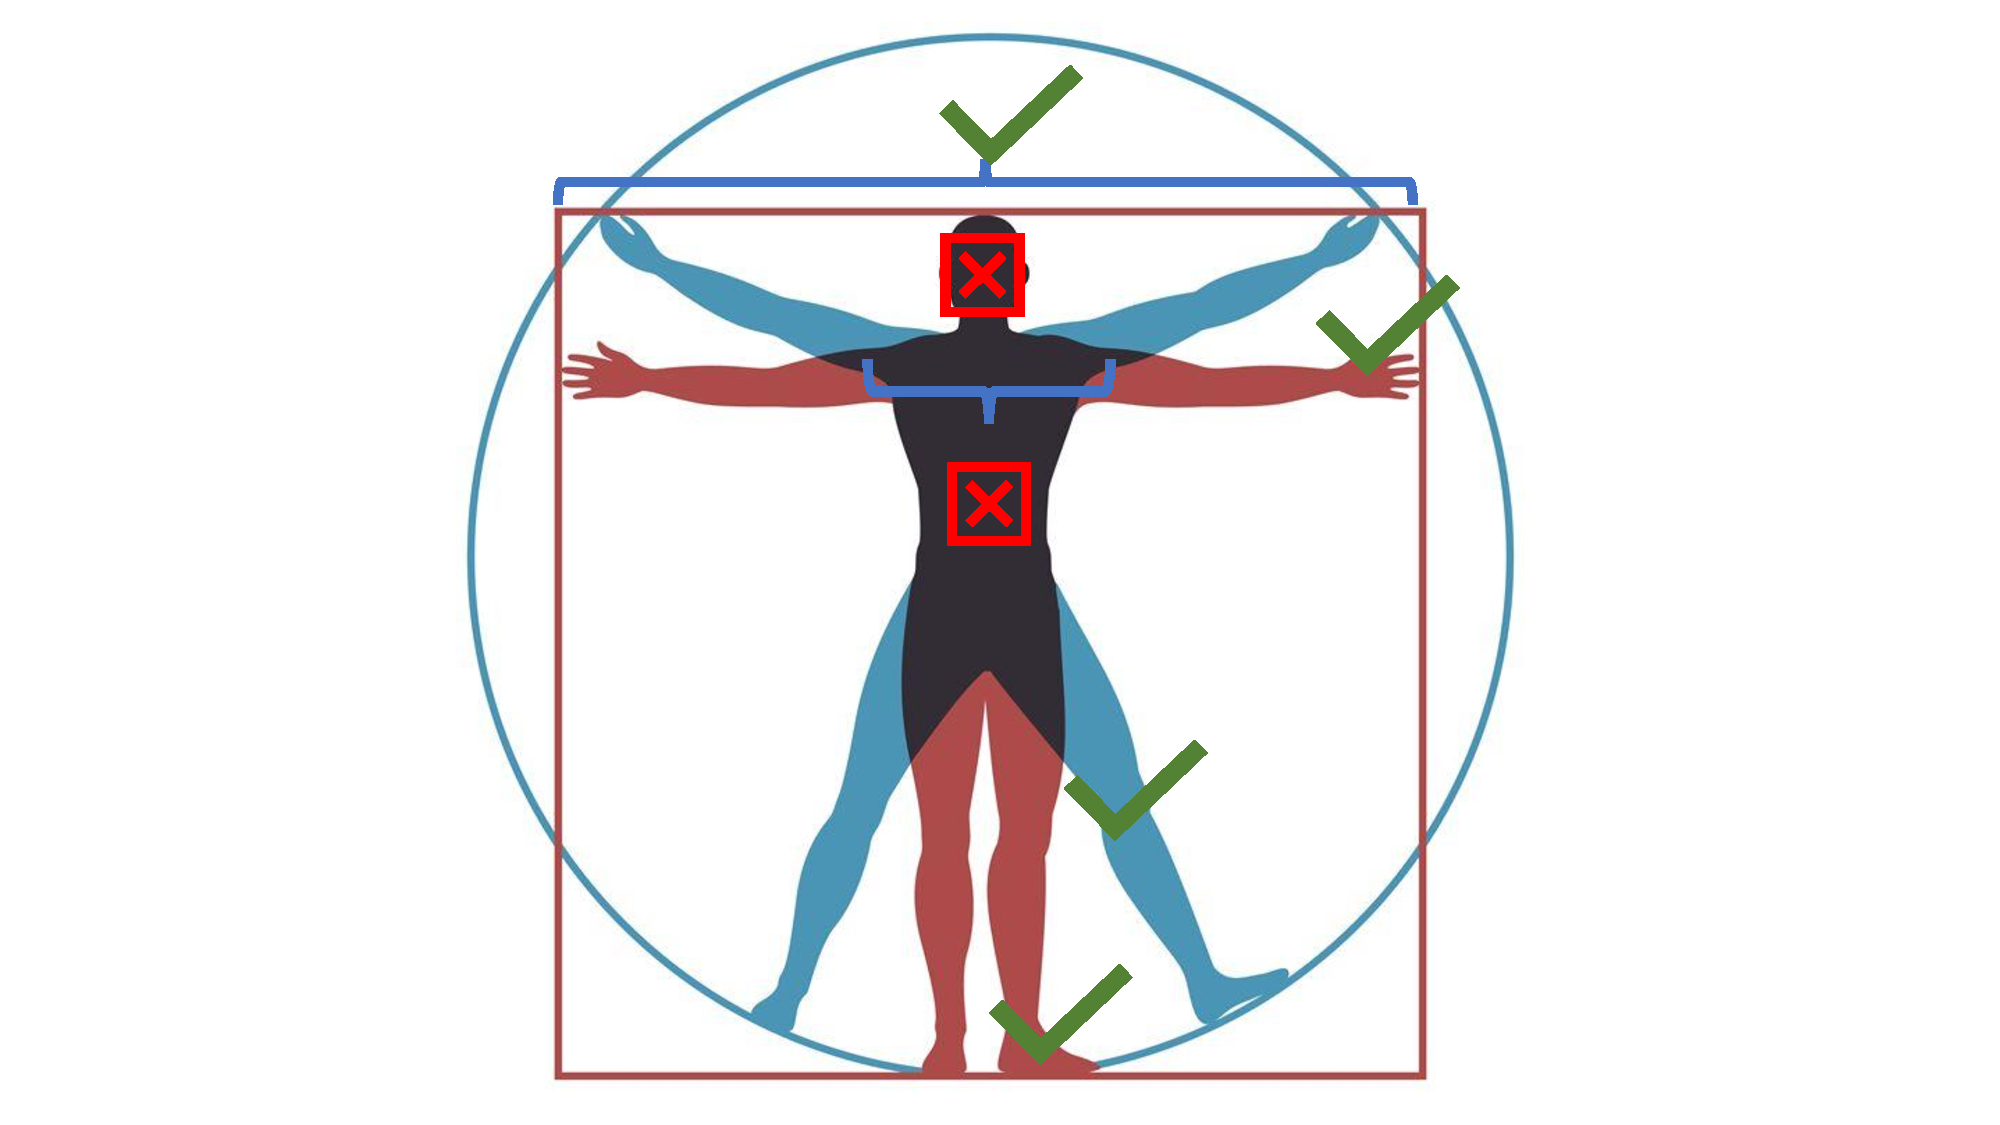
\includegraphics[clip,scale=0.4]{figures/one_graphic.pdf}
        \caption{ True Vitruvian Proportions}
        \label{fig:one-graphic}
\end{figure}

\begin{quote}
"the open hand from the wrist to the tip of the middle finger is [a tenth part of the whole height]; the head from the chin to the crown is an eighth, ... The length of the foot is one sixth of the height of the body... and the breadth of the breast is also one fourth... outstretched arms... will be found to be the same as the height"
\end{quote}

\citep{Vitruvius}

\section{Research Question:  Are the Vitruvian Man proportions realistic?}
\label{sec:rq}

Below is the table with the proportions set out by Vitruvius that we can
investigate with the data that we have. I am interested to see if these
proportions are accurate by comparing them to the results that we have
gathered.

\begin{center}
\begin{tabular}{ l c}
  \label{tab:vitruvian-props}
  \textbf{Body length} & \textbf{Vitruvian Man proportions}\\
  \hline
  Head height & 0.125\\
  Arm span & 1.000\\
  Hand length & 0.100\\
  Foot length & 0.167\\
  Knee height & 0.250\\
  Shoulder width & 0.250\\
\end{tabular}
\end{center}
\subsection{What measurement besides height explains the most body proportions for?}
\label{sec:rq2}

Height is one of the easiest measurements to relate the size of other
body parts to. It would be interesting to know what other measurements
we could use as a substitute. This way if we did not know someone's
height we might be able to make some observations anyway.

\subsection{Do body proportions differ significantly between males and females?}

Vitruvius and DaVinci only considered the proportions of males when they
constructed the ideal body proportions. I am interested if the
proportions for females are the same as for males. If they are not,
which ones differ the most. \label{sec:rq3}

\section{Data Description}
\label{sec:data}

The data was collected by approximately 30 students who are enrolled in
STAT 419 at WSU. Students were supposed to gather measurements from at
least ten people. The measurements gathered were: height, head height,
head circumference, arm span, floor to navel, hand length, hand width,
hand to elbow, elbow to armpit, arm reach, foot length, floor to
knee-pit\footnote{The terms knee-pit and knee height may be used interchangably throughout},
floor to hip, and floor to armpit. The measurements were collected by
having either the student or another measure the subject with a
measuring tape such as the ones used by tailors. Students were also
asked to record which side of the body the measurements came from. Some
students chose to gather measurements from both sides for the sake of
completeness. \newline\newline The data from all students was then
compiled into one dataset. The total dataset contains 263 rows of
measurements. Covariates for each row were also collected. Each subject
was instructed to identify their writing hand, swinging hand, dominant
eye, eye color, age, gender, and ethnicity. The data collector then
assigned a value (1-10) assessing the quality of the measurements taken,
and recorded the amount of minutes that it took to complete the
measurements.

\newpage
\subsection{Summary of Sample}
\label{sec:data-sample}

The sample contained about equal parts male and female subjects.
Subjects identifying as white made up about 70\% of the dataset, the
next largest ethnicity was Asian, which contained about 15\% of
subjects. The majority of those sampled were in their 20s. There were
not many under 10 or over 70 sampled. Subjects who preferred their
right-side made up about 80\% of the sample. Most subjects had brown or
blue eyes --46 and 31 percent respectively-- with a a lesser number of
hazel or green eyed persons. The quality of the data collected ranged
mostly between 8-10 on a 10-point scale. Most data collectors took
between 10-20 minutes to gather all measurements required.

\begin{figure}[!ht]
    \begin{subfigure}[h]{0.5\textwidth}
    \centering
    %  trim={<left> <lower> <right> <upper>}
    % https://shantoroy.com/latex/add-subfig-in-latex/
            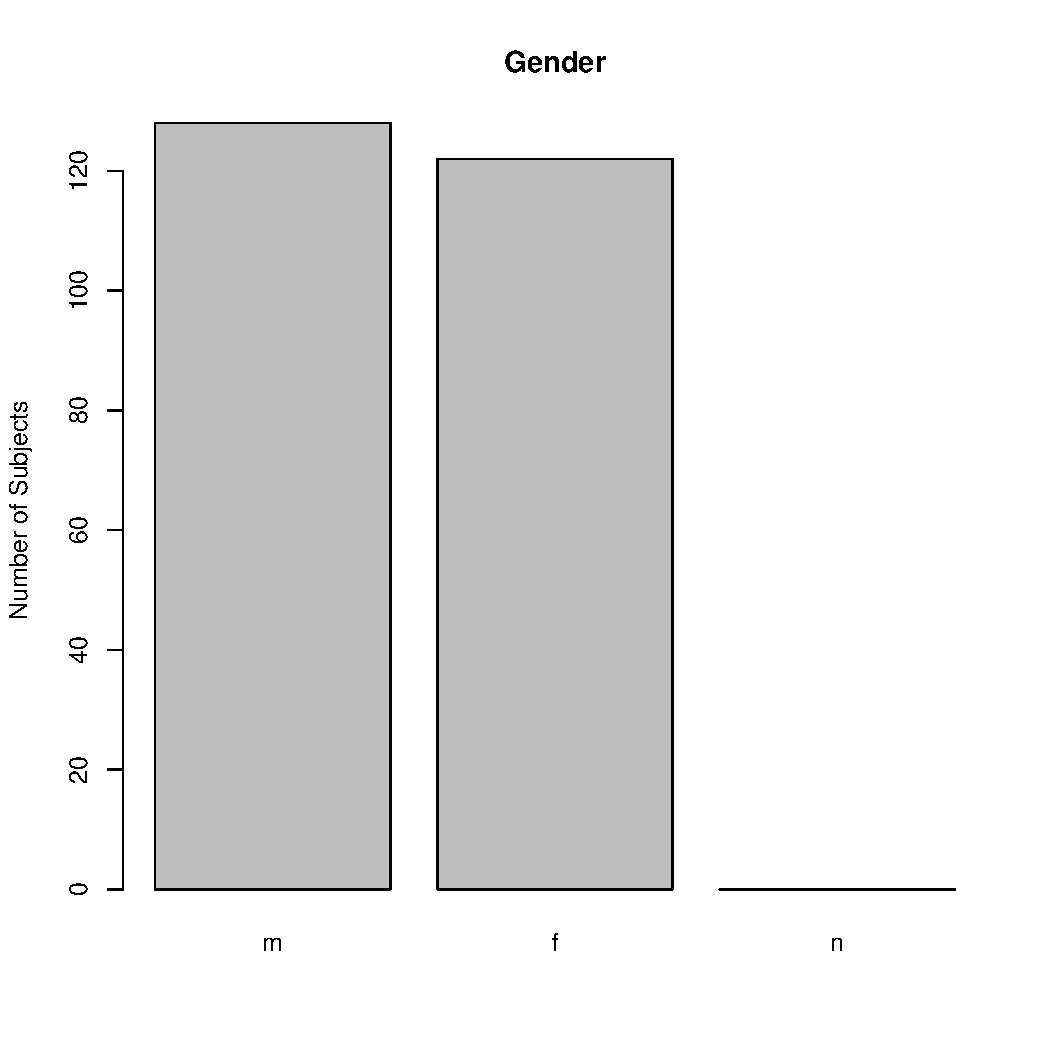
\includegraphics[clip,scale=0.4]{figures/gender-plot.pdf}
        \caption{ Gender Distribution}
        \label{fig:gender-plot}
    \end{subfigure}
    \begin{subfigure}[h]{0.5\textwidth}
    \centering
        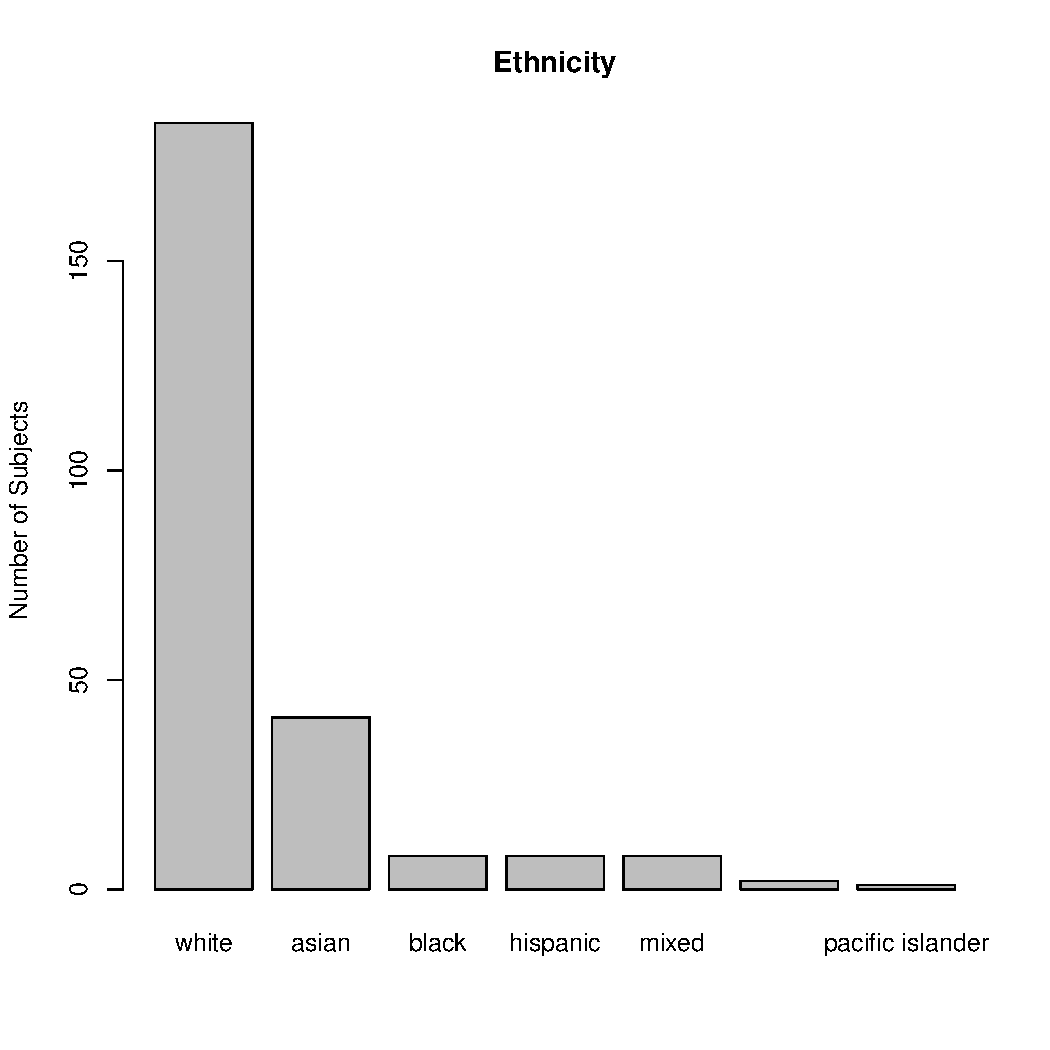
\includegraphics[clip,scale=0.4]{figures/ethnicity-plot.pdf}
            \caption{Ethnicity Distribution}
        \label{fig:ethnicity-plot}
    \end{subfigure}
    \vspace{2.5mm}
    \hrule
    \vspace{2.5mm}
        \caption{\textbf{ Gender and Ethnicity Distributions } }
        \label{fig:ge-plot}
\end{figure}

\newpage
\subsection{Summary Statistics of Data}
\label{sec:data-summary}

By comparing tables below we can see that the average proportion for
both male and female subjects are about the same. However, the standard
deviations show that males vary more in arm span and shoulder width. To
a lesser extent males vary more with hand length as well. Females have a
more variable head.height proportion. Females also have a slightly more
variable foot length and floor to knee-pit length.

\begin{table}[!htbp]
\footnotesize
\centering
\caption{\textbf{Descriptive Statistics and Correlation Analysis (FEMALE)}}
\label{table:correlation-female}
\begin{tabularx}{1\textwidth}{{r@{ \ \ } p{30mm} r@{}lp{1mm} r@{}l p{5mm} r@{}l p{2mm} r@{}l p{2mm} r@{}l p{2mm} r@{}l p{2mm} r@{}l p{2mm}   r@{}l  }}
 & \\
\hline
 & \\
\multicolumn{2}{c}{\textbf{ }} & \multicolumn{2}{c}{\textbf{M}} & & \multicolumn{2}{c}{\textbf{SD}} &  & \multicolumn{2}{c}{\textbf{1}} &  & \multicolumn{2}{c}{\textbf{2}} &  & \multicolumn{2}{c}{\textbf{3}} &  & \multicolumn{2}{c}{\textbf{4}} &  & \multicolumn{2}{c}{\textbf{5}} &  & \\ 
 & \\
\hline
 & \\
\textbf{1} & \textbf{head.height} &  &.133 &  &  &.017 &  &  1&  &  &  \multicolumn{2}{c}{ \  \  \  \  \ }  &  &  \multicolumn{2}{c}{ \  \  \  \  \ }  &  &  \multicolumn{2}{c}{ \  \  \  \  \ }  &  &  \multicolumn{2}{c}{ \  \  \  \  \ }  &  & \\ 
 & \\
\textbf{2} & \textbf{arm.span} &  1&.008 &  &  &.050 &  &  -&.04 &  &  1&  &  &  \multicolumn{2}{c}{ \  \  \  \  \ }  &  &  \multicolumn{2}{c}{ \  \  \  \  \ }  &  &  \multicolumn{2}{c}{ \  \  \  \  \ }  &  & \\ 
 & \\
\textbf{3} & \textbf{hand.length} &  &.108 &  &  &.007 &  &  &.30{$^{**}$}  &  &  &.03 &  &  1&  &  &  \multicolumn{2}{c}{ \  \  \  \  \ }  &  &  \multicolumn{2}{c}{ \  \  \  \  \ }  &  & \\ 
 & \\
\textbf{4} & \textbf{foot.length} &  &.145 &  &  &.010 &  &  &.22{$^{*}$}  &  &  &.18{$^{\dagger}$}  &  &  &.48{$^{***}$}  &  &  1&  &  &  \multicolumn{2}{c}{ \  \  \  \  \ }  &  & \\ 
 & \\
\textbf{5} & \textbf{floor.kneepit} &  &.267 &  &  &.019 &  &  &.12 &  &  &.06 &  &  &.29{$^{**}$}  &  &  &.30{$^{**}$}  &  &  1&  &  & \\ 
 & \\
\textbf{6} & \textbf{shoulder.width} &  &.186 &  &  &.065 &  &  &.01 &  &  &.55{$^{***}$}  &  &  -&.06 &  &  -&.04 &  &  -&.10 &  & \\ 
 & \\
\hline
 & \\
\multicolumn{22}{p{0.9\textwidth}}{  \footnotesize { \begin{hangparas}{0.75in}{1} \textbf{\underline{Notes}:} \ \ Pearson pairwise correlations are reported; \newline a two-side test was performed to report correlation significance.  \end{hangparas} } }  & \\  
\multicolumn{22}{p{0.9\textwidth}}{  {\tiny {$^{\dagger} p < .10$} }  {     } {\tiny        {$^{*} p < .05$} }  {     } {\tiny       {$^{**} p < .01$} }  {     } {\tiny      {$^{***} p < .001$} } {     }     } & \\ 
 & \\
\hline
\end{tabularx}
\end{table}

\begin{table}[!htbp]
\footnotesize
\centering
\caption{\textbf{Descriptive Statistics and Correlation Analysis (MALE)}}
\label{table:correlation-male}
\begin{tabularx}{1\textwidth}{{r@{ \ \ } p{30mm} r@{}lp{1mm} r@{}l p{5mm} r@{}l p{2mm} r@{}l p{2mm} r@{}l p{2mm} r@{}l p{2mm} r@{}l p{2mm}   r@{}l  }}
 & \\
\hline
 & \\
\multicolumn{2}{c}{\textbf{ }} & \multicolumn{2}{c}{\textbf{M}} & & \multicolumn{2}{c}{\textbf{SD}} &  & \multicolumn{2}{c}{\textbf{1}} &  & \multicolumn{2}{c}{\textbf{2}} &  & \multicolumn{2}{c}{\textbf{3}} &  & \multicolumn{2}{c}{\textbf{4}} &  & \multicolumn{2}{c}{\textbf{5}} &  & \\ 
 & \\
\hline
 & \\
\textbf{1} & \textbf{head.height} &  &.130 &  &  &.013 &  &  1&  &  &  \multicolumn{2}{c}{ \  \  \  \  \ }  &  &  \multicolumn{2}{c}{ \  \  \  \  \ }  &  &  \multicolumn{2}{c}{ \  \  \  \  \ }  &  &  \multicolumn{2}{c}{ \  \  \  \  \ }  &  & \\ 
 & \\
\textbf{2} & \textbf{arm.span} &  1&.011 &  &  &.062 &  &  -&.28{$^{**}$}  &  &  1&  &  &  \multicolumn{2}{c}{ \  \  \  \  \ }  &  &  \multicolumn{2}{c}{ \  \  \  \  \ }  &  &  \multicolumn{2}{c}{ \  \  \  \  \ }  &  & \\ 
 & \\
\textbf{3} & \textbf{hand.length} &  &.109 &  &  &.008 &  &  &.36{$^{***}$}  &  &  -&.09 &  &  1&  &  &  \multicolumn{2}{c}{ \  \  \  \  \ }  &  &  \multicolumn{2}{c}{ \  \  \  \  \ }  &  & \\ 
 & \\
\textbf{4} & \textbf{foot.length} &  &.148 &  &  &.009 &  &  &.14 &  &  -&.07 &  &  &.52{$^{***}$}  &  &  1&  &  &  \multicolumn{2}{c}{ \  \  \  \  \ }  &  & \\ 
 & \\
\textbf{5} & \textbf{floor.kneepit} &  &.267 &  &  &.018 &  &  &.26{$^{**}$}  &  &  -&.20{$^{*}$}  &  &  &.05 &  &  &.16{$^{\dagger}$}  &  &  1&  &  & \\ 
 & \\
\textbf{6} & \textbf{shoulder.width} &  &.203 &  &  &.092 &  &  -&.14 &  &  &.55{$^{***}$}  &  &  -&.16 &  &  -&.15 &  &  -&.08 &  & \\ 
 & \\
\hline
 & \\
\multicolumn{22}{p{0.9\textwidth}}{  \footnotesize { \begin{hangparas}{0.75in}{1} \textbf{\underline{Notes}:} \ \ Pearson pairwise correlations are reported; \newline a two-side test was performed to report correlation significance.  \end{hangparas} } }  & \\  
\multicolumn{22}{p{0.9\textwidth}}{  {\tiny {$^{\dagger} p < .10$} }  {     } {\tiny        {$^{*} p < .05$} }  {     } {\tiny       {$^{**} p < .01$} }  {     } {\tiny      {$^{***} p < .001$} } {     }     } & \\ 
 & \\
\hline
\end{tabularx}
\end{table}


Male and female subjects have the significant positive correlations for
hand length and head height, shoulder width and arm span, and foot
length and hand length. This means that for any person if they have
wider shoulders, then they are likely to have a bigger arm span. If a
person has longer hands they are more likely to have a taller head and
longer feet. For male subjects there is also a negative correlation
between arm span and head height, meaning that those with bigger arm
spans are likely to have shorter heads. However, there is a positive
correlation for males between the height of the knee and the height of
the head, meaning that a male with a higher knee (or longer legs?) is
more likely to have a longer head. For female subjects there are
significant positive correlations between the height of the knee, and
both hand length and foot length. This suggests that females with longer
legs may have longer feet and hands.

\section{Key Findings}
\label{sec:findings}

From running several t-tests on the male proportion data we can find
which proportions align with the Vitruvian man. From the tests it seems
that only arm span might be correct. The Vitruvian proportions for head
height, hand length and knee height seem to be underestimated. In
contrast the foot length and shoulder width data may have been
overestimated.
\footnote{Our shoulder width data was computed by subtracting two times the length of the arm from the arm span. This gives the inner width of shoulders which likely differs from the method used by Vitruvius.}
Even though most of the Vitruvian proportions seem to disagree with
where the true average might be, they are remarkably close to where the
true average probably lies. In most cases, our measurements are not off
by more than about 3\% of the Vitruvian measurements. The two exceptions
are shoulder width, and head height. \newline\newline We have also found
that the proportions for male and female subjects do not differ
significantly for any of the variables except for foot length. For males
the proportion of foot length to height is significantly larger than the
same measurement for females. Testing the height of the knee especially
shows that the male and female measurements are likely to be almost the
same. \newline\newline From the earlier calculations of the correlations
we can determine that hand length is the best measurement for relating
other measurements for either male or female subjects. For female
subjects knee height also helps a lot to explain other proportions. For
male subjects, the head height variable can also explain other
proportions.

\begin{figure}[!ht]
    \begin{subfigure}[h]{0.5\textwidth}
    \centering
    %  trim={<left> <lower> <right> <upper>}
    % https://shantoroy.com/latex/add-subfig-in-latex/
            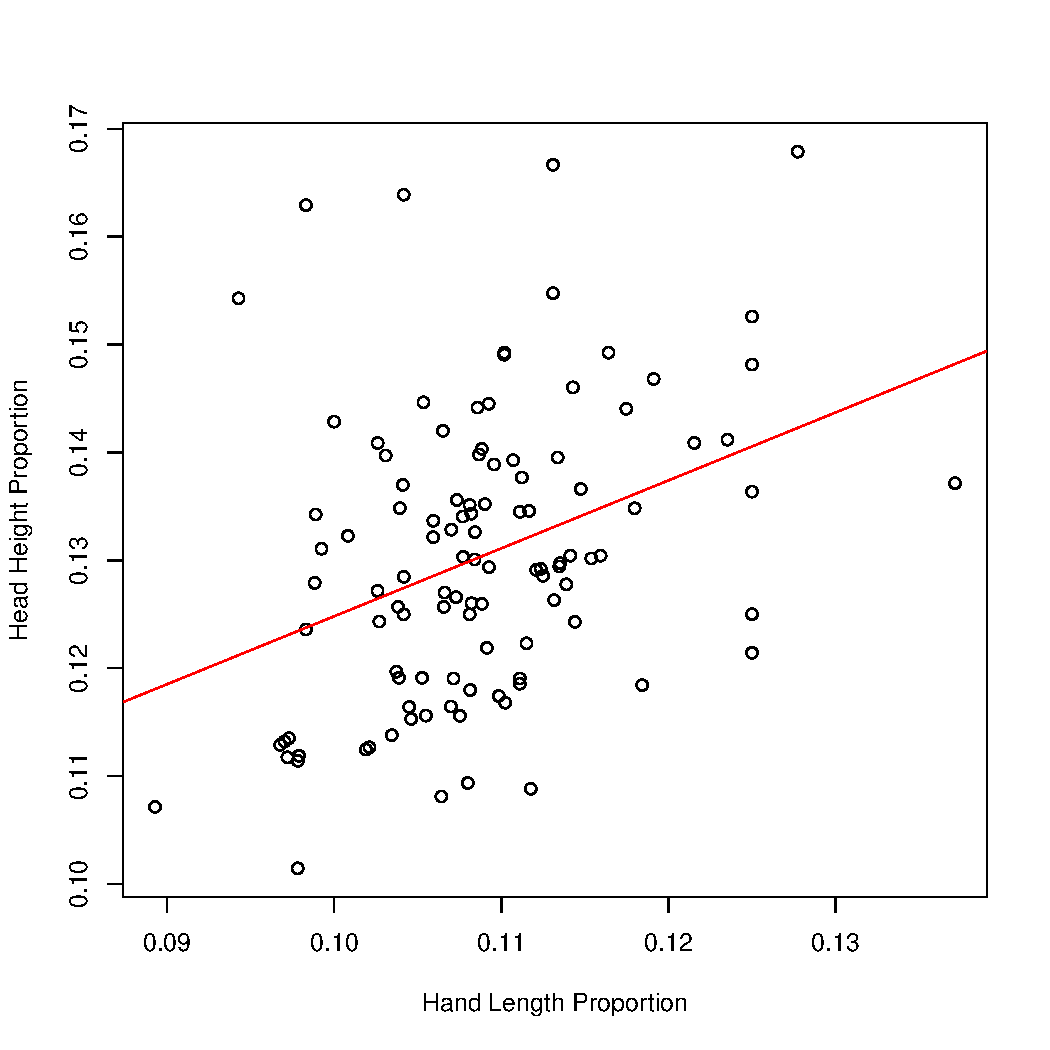
\includegraphics[clip,scale=0.5]{figures/hand-length-head-height-plot.pdf}
        \caption{ Hand Length - Head Length Relationship}
        \label{fig:hand-head-plot}
    \end{subfigure}
    \begin{subfigure}[h]{0.5\textwidth}
    \centering
        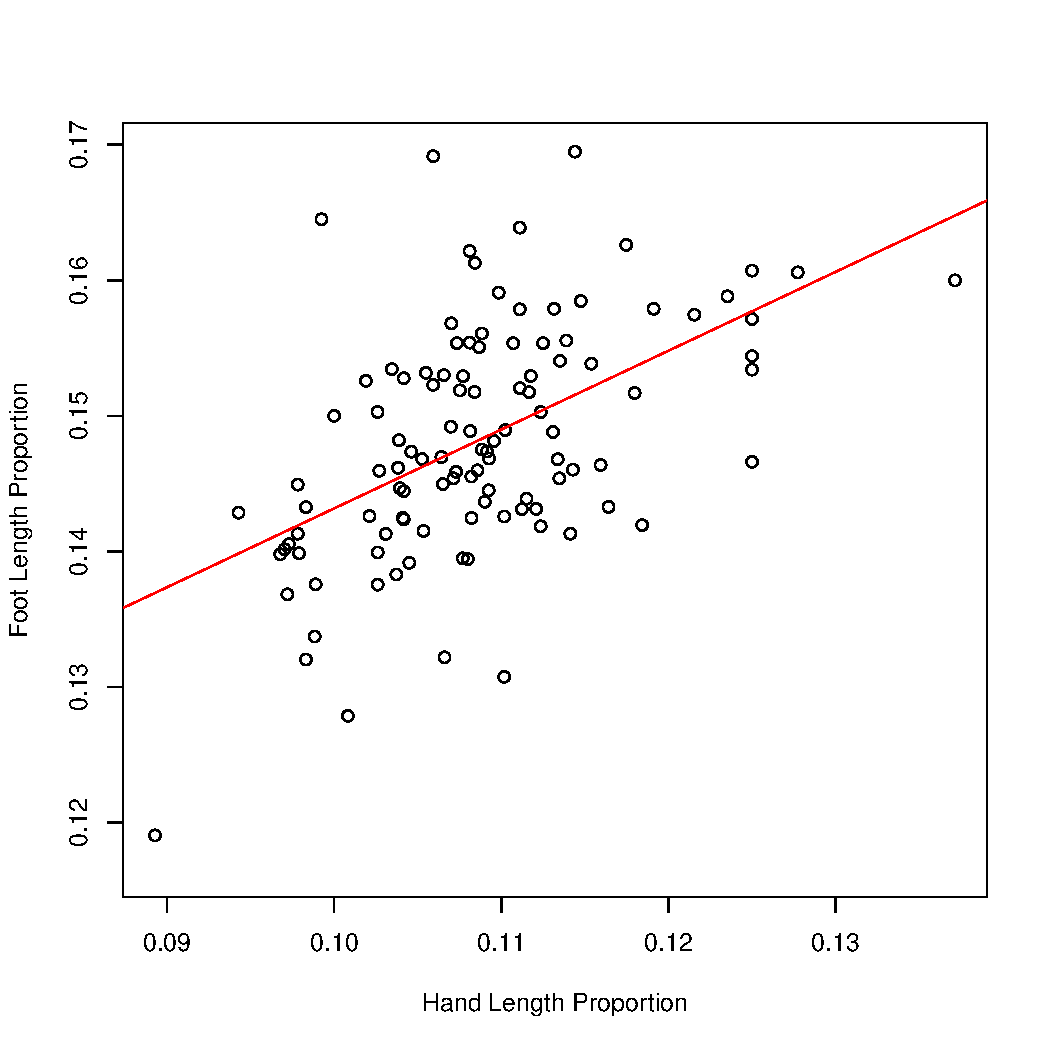
\includegraphics[clip,scale=0.5]{figures/hand-length-foot-length.pdf}
            \caption{Hand Length - Foot Length Relationship}
        \label{fig:hand-foot-plot}
    \end{subfigure}
    \vspace{2.5mm}
    \hrule
    \vspace{2.5mm}
        \caption{\textbf{ Hand Length Relationships } }
        \label{fig:hand-plots}
\end{figure}

\newpage
\section{Conclusion}
\label{sec:conclusion}

From our findings in Section \ref{sec:findings} we can conclude that arm
span, hand length, foot length, and the knee height are all consistent
with the Vitruvian measures.
\footnote{Consistent here means that our measurement proportions are within 3\% of the Vitruvian proportions.}
The same cannot be said for head height which is larger than the
Vitruvian proportions, and for shoulder width, which is smaller than the
Vitruvian proportions. \newline\newline In our investigation of male and
female subjects we are able to conclude that in most respects the
Vitruvian proportions hold for females as well as they do for males. The
one notable exception being foot length, which is larger in males than
in females. \newline\newline Lastly, I have determined from Section
\ref{sec:findings} that the hand length proportion can be used in
determining the other proportions of a human body. From Section
\ref{sec:data-summary} I have also determined that in the case of female
subjects, the knee height proportion can help in determining other
proportions. Likewise, for male subjects, the head height proportion can
help in determining other proportions. \newline\newline The conclusions
here may not be able to be generalized widely due the the lack of ethnic
diversity present in the sample as seen in Figure
\ref{fig:ethnicity-plot}. The range of ages for this dataset was also
overwhelmingly of subjects in theirs 20s. Those wishing to improve the
results of this study should seek to diversify the samples to be able to
make more confident generalizations of body proportions.

\newpage
\section{APPENDICES}
\label{sec:appendix}

\subsection{Data Provenance}
\label{sec:appendix-data-provenance}

As was listed in Section \ref{sec:data} the data collection was assigned
to the STAT 419 class at WSU, which is around 30 people. This can lead
to some discrepancies in the way that the data was collected. The data
may not always have been measured by students, but by the people which
their handouts were sent to. For the 10 people that I gathered
measurements for I measured seven people personally, and then had three
others send me their results by email. The number of data collectors
involved can also lead to different interpretations of what each
measurement means. \newline\newline The data collector was given the
option to pick which units they wished to measure in, and the subject
was also asked to identify their preferred hand in writing and swinging,
what eye is dominant, what their eye color is, how old they are, what
gender they are, and what ethnicity they identify as. These covariates
give us a better picture of our sample. For example, since we have about
equal amounts of male and female measurements (\ref{fig:gender-plot}) we
can make some generalizations. But on the other hand, we do not have
much diversity of ethnicity in subjects (\ref{fig:ethnicity-plot}) so we
can not generalize our results as easily. \newline\newline Some of the
measurements seemed like they had more outliers than others. This is
likely because they were either entered incorrectly or they were
measured differently. The measurements with significant outliers are:
hand length, arm reach, floor to knee-pit, and head height. Hand length
was supposed to be measured from the tip of the middle finger to the
wrist. Arm reach is supposed to be the measurement from the floor to the
tip of the middle finger when the arms are pointed upwards above the
head. The floor to knee-pit measurement is from the heel to the back of
knee. Lastly the head height measurement is from the chin to the top of
the head. \newline\newline Below shows the handout I used to conduct my
measurements and which was sent to those whom I could not personally
measure. \newpage

\subsubsection{Data Collection Handout}
\label{sec:appendix-data-handout}

\begin{figure}[!ht]
    \hrule
    \caption{ \textbf{Handout Page 1} }
    \begin{center}
        \scalebox{1.00}{    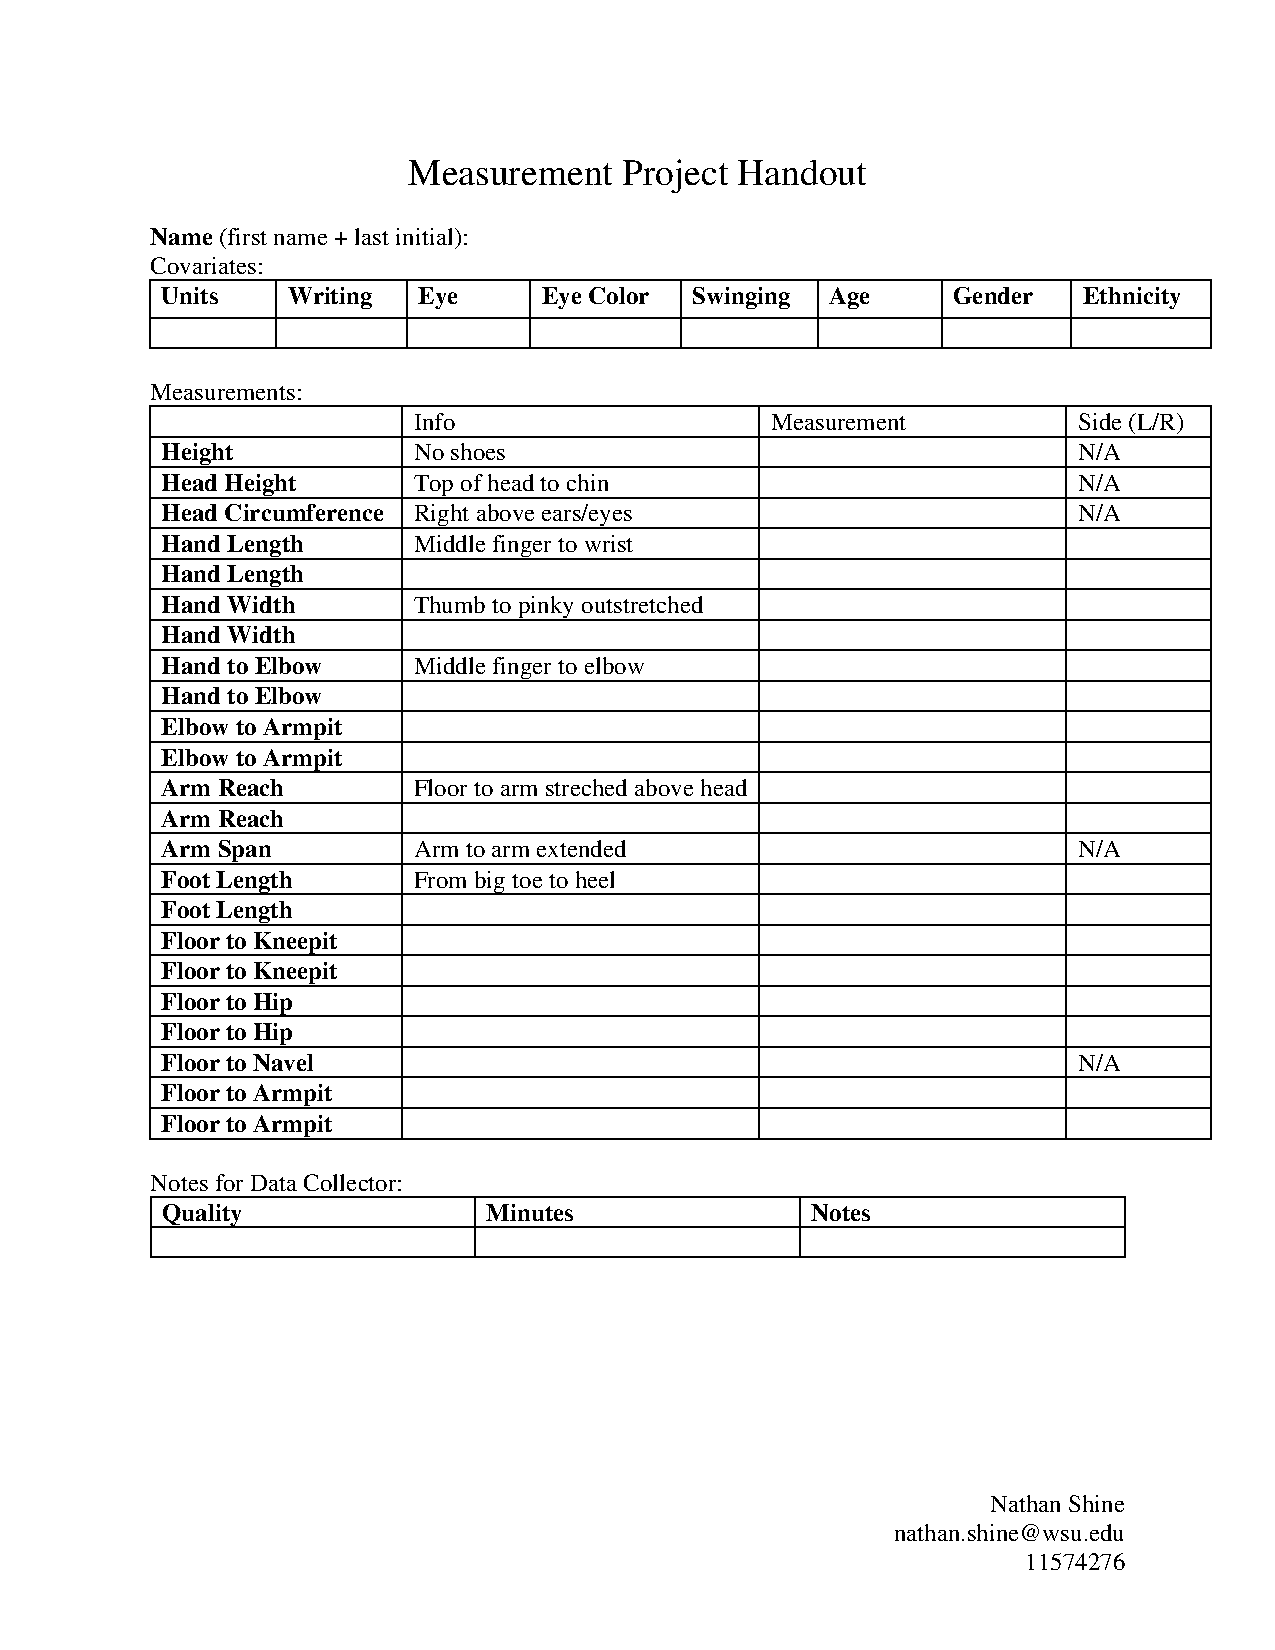
\includegraphics[trim = 0 0 0 0,clip,width=0.85\textwidth]{pdfs/shine_handout.pdf} }
    \end{center}
    \label{fig:handout-1}
    \hrule
\end{figure}

\newpage

\subsection{Preparing the Report Workspace}
\label{sec:appendix-setup}

\subsubsection{Preparing the Data}
\label{sec:appendix-data-prep}

Below is the necessary functions and libraries required to run the code
referenced in this document.

\begin{Shaded}
\begin{Highlighting}[]
\FunctionTok{library}\NormalTok{(devtools);       }\CommentTok{\# required for source\_url}

\NormalTok{path.humanVerseWSU }\OtherTok{=} \StringTok{"https://raw.githubusercontent.com/MonteShaffer/humanVerseWSU/"}
\FunctionTok{source\_url}\NormalTok{( }\FunctionTok{paste0}\NormalTok{(path.humanVerseWSU,}\StringTok{"master/misc/functions{-}project{-}measure.R"}\NormalTok{) );}
\end{Highlighting}
\end{Shaded}

Below is the code to load the data and prepare it for analysis.

\begin{Shaded}
\begin{Highlighting}[]
\NormalTok{path.to.secret }\OtherTok{=} \StringTok{"C:/Users/Nathan/Dropbox/\_\_student\_access\_\_/\_SECRET\_/"}\NormalTok{;}

\NormalTok{measure }\OtherTok{=}\NormalTok{ utils}\SpecialCharTok{::}\FunctionTok{read.csv}\NormalTok{( }\FunctionTok{paste0}\NormalTok{(path.to.secret, }\StringTok{"measure{-}students.txt"}\NormalTok{), }
                           \AttributeTok{header=}\ConstantTok{TRUE}\NormalTok{, }\AttributeTok{quote=}\StringTok{""}\NormalTok{, }\AttributeTok{sep=}\StringTok{"|"}\NormalTok{);}
\NormalTok{path.my.github }\OtherTok{=} \StringTok{"https://raw.githubusercontent.com/nshine787/WSU\_STATS419\_FALL2020/"}\NormalTok{;}
\FunctionTok{source\_url}\NormalTok{(}\FunctionTok{paste0}\NormalTok{(path.my.github, }\StringTok{\textquotesingle{}master/functions/functions{-}project{-}measure.R\textquotesingle{}}\NormalTok{))}

\NormalTok{relevantColumns }\OtherTok{=} \FunctionTok{c}\NormalTok{(}\StringTok{\textquotesingle{}height\textquotesingle{}}\NormalTok{, }\StringTok{\textquotesingle{}head.height\textquotesingle{}}\NormalTok{,}\StringTok{\textquotesingle{}arm.span\textquotesingle{}}\NormalTok{,}\StringTok{\textquotesingle{}}
\StringTok{                    hand.length\textquotesingle{}}\NormalTok{,}\StringTok{\textquotesingle{}foot.length\textquotesingle{}}\NormalTok{,}\StringTok{\textquotesingle{}floor.kneepit\textquotesingle{}}\NormalTok{,}\StringTok{\textquotesingle{}shoulder.width\textquotesingle{}}\NormalTok{)}
\NormalTok{measure.df }\OtherTok{=} \FunctionTok{prepareMeasureData}\NormalTok{(measure);}
\NormalTok{measure.males.df }\OtherTok{=} \FunctionTok{grabGenderRows}\NormalTok{(measure.df,}\StringTok{\textquotesingle{}m\textquotesingle{}}\NormalTok{)[,relevantColumns]}
\NormalTok{measure.females.df }\OtherTok{=} \FunctionTok{grabGenderRows}\NormalTok{(measure.df,}\StringTok{\textquotesingle{}f\textquotesingle{}}\NormalTok{)[,relevantColumns]}

\NormalTok{proportions.male }\OtherTok{=}\NormalTok{ measure.males.df}\SpecialCharTok{/}\NormalTok{measure.males.df}\SpecialCharTok{$}\NormalTok{height}
\NormalTok{proportions.female }\OtherTok{=}\NormalTok{ measure.females.df}\SpecialCharTok{/}\NormalTok{measure.females.df}\SpecialCharTok{$}\NormalTok{height}
\end{Highlighting}
\end{Shaded}

\subsubsection{Creating Figures}
\label{sec:appendix-create-figures}

The code below shows the distributions of gender and ethnicity in the
sample as seen in Figure \ref{fig:ge-plot}

\begin{Shaded}
\begin{Highlighting}[]
\FunctionTok{barplot}\NormalTok{(}\FunctionTok{sort}\NormalTok{(}\FunctionTok{table}\NormalTok{(measure.df}\SpecialCharTok{$}\NormalTok{ethnicity),}\AttributeTok{decreasing=}\ConstantTok{TRUE}\NormalTok{), }\AttributeTok{main =} \StringTok{\textquotesingle{}Ethnicity\textquotesingle{}}\NormalTok{,}
        \AttributeTok{ylab =} \StringTok{\textquotesingle{}Number of Subjects\textquotesingle{}}\NormalTok{)}
\FunctionTok{barplot}\NormalTok{(}\FunctionTok{sort}\NormalTok{(}\FunctionTok{table}\NormalTok{(measure.df}\SpecialCharTok{$}\NormalTok{gender),}\AttributeTok{decreasing=}\ConstantTok{TRUE}\NormalTok{), }\AttributeTok{main =} \StringTok{\textquotesingle{}Gender\textquotesingle{}}\NormalTok{, }
        \AttributeTok{ylab =} \StringTok{\textquotesingle{}Number of Subjects\textquotesingle{}}\NormalTok{)}
\end{Highlighting}
\end{Shaded}

Below is the code to generate the summary statistics and save them as a
table that you see in Section \ref{sec:data-summary}. It uses a function
created by Monte Shaffer, the instructor of the STAT 419 class at WSU.

\begin{Shaded}
\begin{Highlighting}[]
\NormalTok{path.tables }\OtherTok{=} \FunctionTok{paste0}\NormalTok{(path.project,}\StringTok{\textquotesingle{}PROJECT{-}01/tables/\textquotesingle{}}\NormalTok{)}
\NormalTok{file.correlation }\OtherTok{=} \FunctionTok{paste0}\NormalTok{(path.tables,}\StringTok{"male{-}correlation{-}table.tex"}\NormalTok{);}

\NormalTok{myData }\OtherTok{=} \FunctionTok{as.matrix}\NormalTok{(proportions.male);}
\NormalTok{myData }\OtherTok{=}\NormalTok{ myData[,}\FunctionTok{c}\NormalTok{(}\DecValTok{2}\NormalTok{,}\DecValTok{4}\NormalTok{,}\DecValTok{6}\NormalTok{,}\DecValTok{11}\NormalTok{,}\DecValTok{12}\NormalTok{,}\DecValTok{15}\NormalTok{)]}

\FunctionTok{buildLatexCorrelationTable}\NormalTok{(myData, }
  \AttributeTok{rotateTable =} \ConstantTok{FALSE}\NormalTok{,}
  \AttributeTok{width.table =} \DecValTok{1}\NormalTok{,}
  \AttributeTok{width.names =} \StringTok{"30mm"}\NormalTok{,}
  \AttributeTok{myFile =}\NormalTok{ file.correlation,}
  \AttributeTok{round.digits =} \FunctionTok{c}\NormalTok{(}\DecValTok{2}\NormalTok{,}\DecValTok{3}\NormalTok{,}\DecValTok{2}\NormalTok{),}
  \AttributeTok{myLabel =} \StringTok{"table:correlation{-}male"}\NormalTok{,}
  \AttributeTok{myCaption =} \StringTok{"Descriptive Statistics and Correlation Analysis (MALE)"}
\NormalTok{  );}
\FunctionTok{Sys.sleep}\NormalTok{(}\DecValTok{2}\NormalTok{);}

\NormalTok{file.correlation }\OtherTok{=} \FunctionTok{paste0}\NormalTok{(path.tables,}\StringTok{"female{-}correlation{-}table.tex"}\NormalTok{);}

\NormalTok{myData }\OtherTok{=} \FunctionTok{as.matrix}\NormalTok{(proportions.female);}
\NormalTok{myData }\OtherTok{=}\NormalTok{ myData[,}\FunctionTok{c}\NormalTok{(}\DecValTok{2}\NormalTok{,}\DecValTok{4}\NormalTok{,}\DecValTok{6}\NormalTok{,}\DecValTok{11}\NormalTok{,}\DecValTok{12}\NormalTok{,}\DecValTok{15}\NormalTok{)]}

\FunctionTok{buildLatexCorrelationTable}\NormalTok{(myData, }
  \AttributeTok{rotateTable =} \ConstantTok{FALSE}\NormalTok{,}
  \AttributeTok{width.table =} \DecValTok{1}\NormalTok{,}
  \AttributeTok{width.names =} \StringTok{"30mm"}\NormalTok{,}
  \AttributeTok{myFile =}\NormalTok{ file.correlation,}
  \AttributeTok{round.digits =} \FunctionTok{c}\NormalTok{(}\DecValTok{2}\NormalTok{,}\DecValTok{3}\NormalTok{,}\DecValTok{2}\NormalTok{),}
  \AttributeTok{myLabel =} \StringTok{"table:correlation{-}female"}\NormalTok{,}
  \AttributeTok{myCaption =} \StringTok{"Descriptive Statistics and Correlation Analysis (FEMALE)"}
\NormalTok{  );}
\FunctionTok{Sys.sleep}\NormalTok{(}\DecValTok{2}\NormalTok{);}
\end{Highlighting}
\end{Shaded}

Below is the code to generate the plots in Section \ref{sec:findings}

\begin{Shaded}
\begin{Highlighting}[]
\NormalTok{proportions.both }\OtherTok{=} \FunctionTok{merge.data.frame}\NormalTok{(myDataMale,myDataFemale,}\AttributeTok{all.x=}\ConstantTok{TRUE}\NormalTok{)}

\FunctionTok{plot}\NormalTok{(proportions.both}\SpecialCharTok{$}\NormalTok{hand.length,proportions.both}\SpecialCharTok{$}\NormalTok{head.height, }
     \AttributeTok{xlab =} \StringTok{\textquotesingle{}Hand Length Proportion\textquotesingle{}}\NormalTok{, }\AttributeTok{ylab=}\StringTok{\textquotesingle{}Head Height Proportion\textquotesingle{}}\NormalTok{)}
\FunctionTok{abline}\NormalTok{(}\FunctionTok{lm}\NormalTok{(proportions.both}\SpecialCharTok{$}\NormalTok{head.height}\SpecialCharTok{\textasciitilde{}}\NormalTok{proportions.both}\SpecialCharTok{$}\NormalTok{hand.length), }\AttributeTok{col=}\StringTok{\textquotesingle{}red\textquotesingle{}}\NormalTok{)}

\FunctionTok{plot}\NormalTok{(proportions.both}\SpecialCharTok{$}\NormalTok{hand.length, proportions.both}\SpecialCharTok{$}\NormalTok{foot.length, }
     \AttributeTok{xlab =} \StringTok{\textquotesingle{}Hand Length Proportion\textquotesingle{}}\NormalTok{, }\AttributeTok{ylab=}\StringTok{\textquotesingle{}Foot Length Proportion\textquotesingle{}}\NormalTok{)}
\FunctionTok{abline}\NormalTok{(}\FunctionTok{lm}\NormalTok{(proportions.both}\SpecialCharTok{$}\NormalTok{foot.length}\SpecialCharTok{\textasciitilde{}}\NormalTok{proportions.both}\SpecialCharTok{$}\NormalTok{hand.length), }\AttributeTok{col=}\StringTok{\textquotesingle{}red\textquotesingle{}}\NormalTok{)}
\end{Highlighting}
\end{Shaded}

\subsubsection{Running the Tests}
\label{sec:appendix-tests}

Below is the code to generate the t-tests in Section \ref{sec:findings}.
The first chunk compares the male proportions to the ideal Vitruvian
proportions. The second chunk tests the male and female observations
against each other for each variable to see if the proportions vary
significantly.

\begin{Shaded}
\begin{Highlighting}[]
\NormalTok{myData }\OtherTok{=}\NormalTok{ proportions.male[,}\FunctionTok{c}\NormalTok{(}\StringTok{\textquotesingle{}head.height\textquotesingle{}}\NormalTok{,}\StringTok{\textquotesingle{}arm.span\textquotesingle{}}\NormalTok{,}\StringTok{\textquotesingle{}hand.length\textquotesingle{}}\NormalTok{,}\StringTok{\textquotesingle{}foot.length\textquotesingle{}}
\NormalTok{                             ,}\StringTok{\textquotesingle{}floor.kneepit\textquotesingle{}}\NormalTok{,}\StringTok{\textquotesingle{}shoulder.width\textquotesingle{}}\NormalTok{)]}
\NormalTok{proportions.vitruvian }\OtherTok{=} \FunctionTok{c}\NormalTok{(}\FloatTok{0.125}\NormalTok{,}\DecValTok{1}\NormalTok{,}\FloatTok{0.1}\NormalTok{,}\FloatTok{0.1666667}\NormalTok{,}\FloatTok{0.25}\NormalTok{,}\FloatTok{0.25}\NormalTok{)}
\ControlFlowTok{for}\NormalTok{ (i }\ControlFlowTok{in} \DecValTok{1}\SpecialCharTok{:}\FunctionTok{dim}\NormalTok{(myData)[}\DecValTok{2}\NormalTok{])}
\NormalTok{\{}
  \FunctionTok{print}\NormalTok{(}\FunctionTok{colnames}\NormalTok{(myData)[i])}
\NormalTok{  test.result }\OtherTok{=} \FunctionTok{t.test}\NormalTok{(myData[,i], }\AttributeTok{mu=}\NormalTok{proportions.vitruvian[i], }\AttributeTok{alternative=}\StringTok{\textquotesingle{}two.sided\textquotesingle{}}\NormalTok{)}
  \FunctionTok{print}\NormalTok{(test.result}\SpecialCharTok{$}\NormalTok{p.value)}
  \FunctionTok{print}\NormalTok{(test.result}\SpecialCharTok{$}\NormalTok{conf.int)}
\NormalTok{  error }\OtherTok{=} \FunctionTok{abs}\NormalTok{(test.result}\SpecialCharTok{$}\NormalTok{conf.int[}\DecValTok{1}\NormalTok{]}\SpecialCharTok{{-}}\NormalTok{test.result}\SpecialCharTok{$}\NormalTok{conf.int[}\DecValTok{2}\NormalTok{])}\SpecialCharTok{/}\NormalTok{proportions.vitruvian[i]}
  \FunctionTok{print}\NormalTok{(}\FunctionTok{paste0}\NormalTok{(}\StringTok{\textquotesingle{}Error percent: \textquotesingle{}}\NormalTok{,error))}
  
\NormalTok{\}}
\end{Highlighting}
\end{Shaded}

\begin{Shaded}
\begin{Highlighting}[]
\NormalTok{myDataMale }\OtherTok{=}\NormalTok{ proportions.male[,}\FunctionTok{c}\NormalTok{(}\StringTok{\textquotesingle{}head.height\textquotesingle{}}\NormalTok{,}\StringTok{\textquotesingle{}arm.span\textquotesingle{}}\NormalTok{,}\StringTok{\textquotesingle{}hand.length\textquotesingle{}}\NormalTok{,}\StringTok{\textquotesingle{}foot.length\textquotesingle{}}\NormalTok{,}
                                 \StringTok{\textquotesingle{}floor.kneepit\textquotesingle{}}\NormalTok{,}\StringTok{\textquotesingle{}shoulder.width\textquotesingle{}}\NormalTok{)]}
\NormalTok{myDataFemale }\OtherTok{=}\NormalTok{ proportions.female[,}\FunctionTok{c}\NormalTok{(}\StringTok{\textquotesingle{}head.height\textquotesingle{}}\NormalTok{,}\StringTok{\textquotesingle{}arm.span\textquotesingle{}}\NormalTok{,}\StringTok{\textquotesingle{}hand.length\textquotesingle{}}\NormalTok{,}\StringTok{\textquotesingle{}foot.length\textquotesingle{}}
\NormalTok{                                     ,}\StringTok{\textquotesingle{}floor.kneepit\textquotesingle{}}\NormalTok{,}\StringTok{\textquotesingle{}shoulder.width\textquotesingle{}}\NormalTok{)]}
\NormalTok{proportions.vitruvian }\OtherTok{=} \FunctionTok{c}\NormalTok{(}\FloatTok{0.125}\NormalTok{,}\DecValTok{1}\NormalTok{,}\FloatTok{0.1}\NormalTok{,}\FloatTok{0.1666667}\NormalTok{,}\FloatTok{0.25}\NormalTok{,}\FloatTok{0.25}\NormalTok{)}
\ControlFlowTok{for}\NormalTok{ (i }\ControlFlowTok{in} \DecValTok{1}\SpecialCharTok{:}\FunctionTok{dim}\NormalTok{(myData)[}\DecValTok{2}\NormalTok{])}
\NormalTok{\{}
  \FunctionTok{print}\NormalTok{(}\FunctionTok{colnames}\NormalTok{(myData)[i])}
\NormalTok{  test.result }\OtherTok{=} \FunctionTok{t.test}\NormalTok{(myDataMale[,i],myDataFemale[,i])}
  \FunctionTok{print}\NormalTok{(test.result}\SpecialCharTok{$}\NormalTok{p.value)}
  \FunctionTok{print}\NormalTok{(test.result}\SpecialCharTok{$}\NormalTok{conf.int)}
\NormalTok{\}}
\end{Highlighting}
\end{Shaded}





%% appendices go here!


\newpage
\theendnotes

%%%%%%%%%%%%%%%%%%%%%%%%%%%%%%%%%%%  biblio %%%%%%%%
\newpage
\begin{auxmulticols}{2}
\singlespacing 
\bibliography{./../biblio/master.bib}

%%%%%%%%%%%%%%%%%%%%%%%%%%%%%%%%%%%  biblio %%%%%%%%
\end{auxmulticols}

\newpage
{
\hypersetup{linkcolor=black}
\setcounter{tocdepth}{3}
\tableofcontents
}



\end{document}